\documentclass[conference]{IEEEtran}
\IEEEoverridecommandlockouts
% The preceding line is only needed to identify funding in the first footnote. If that is unneeded, please comment it out.
%Template version as of 6/27/2024

\usepackage{cite}
\usepackage{amsmath,amssymb,amsfonts}
\usepackage{algorithmic}
\usepackage{graphicx}
\usepackage{textcomp}
\usepackage{xcolor}
\usepackage[caption=false,font=footnotesize]{subfig}
\def\BibTeX{{\rm B\kern-.05em{\sc i\kern-.025em b}\kern-.08em
    T\kern-.1667em\lower.7ex\hbox{E}\kern-.125emX}}
\begin{document}

\title{rs1Wire: An Efficient Rust Ecosystem for 1-Wire Thermal Sensors\\
{\footnotesize \textsuperscript{*}Note: Sub-titles are not captured for https://ieeexplore.ieee.org  and
should not be used}
\thanks{Identify applicable funding agency here. If none, delete this.}
}

\author{\IEEEauthorblockN{1\textsuperscript{st} David Costa}
\IEEEauthorblockA{\textit{School of Computing and Data Science} \\
\textit{Wentworth Institute of Technology}\\
Boston, Massachusetts, United States\\
costad3@wit.edu}
\and
\IEEEauthorblockN{2\textsuperscript{nd} Ashar Neyaz}
\IEEEauthorblockA{\textit{School of Computing and Data Science} \\
\textit{Wentworth Institute of Technology}\\
Boston, Massachusetts, United States\\
neyaza@wit.edu}
}

\maketitle

\begin{abstract}
This document is a model and instructions for \LaTeX.
This and the IEEEtran.cls file define the components of your paper [title, text, heads, etc.]. *CRITICAL: Do Not Use Symbols, Special Characters, Footnotes, 
or Math in Paper Title or Abstract.
\end{abstract}

\begin{IEEEkeywords}
component, formatting, style, styling, insert.
\end{IEEEkeywords}

\section*{Introduction}
INTRODUCTION INTRODUCTION INTRODUCTION INTRODUCTION INTRODUCTION INTRODUCTION INTRODUCTION INTRODUCTION INTRODUCTION INTRODUCTION INTRODUCTION INTRODUCTION INTRODUCTION INTRODUCTION INTRODUCTION INTRODUCTION

\subsection{Subsection 1}

More asdfasdfasdfasdfasdfasdfasdfasfasdfasdf\\ details asdfasdfasdfasdfasdfasdfasdfasfasdfasdf\\ about asdfasdfasdfasdfasdfasdfasdfasfasdfasdf\\ Subsection asdfasdfasdfasdfasdfasdfasdfasfasdfasdf\\ 1 asdfasdfasdfasdfasdfasdfasdfasfasdfasdf\\ go asdfasdfasdfasdfasdfasdfasdfasfasdfasdf\\ here asdfasdfasdfasdfasdfasdfasdfasfasdfasdf.

\subsection{Abbreviations and Acronyms}\label{AA}
Define abbreviations and acronyms the first time they are used in the text, 
even after they have been defined in the abstract. Abbreviations such as 
IEEE, SI, MKS, CGS, ac, dc, and rms do not have to be defined. Do not use 
abbreviations in the title or heads unless they are unavoidable.

\section*{Related Work}
Discuss related work ie: python modules and rust crates here. Make sure to explain what the differences and advantages/disadvantages of each are. Explain where the gap lies and what this crate does to address it.

\subsection{Python}


\subsection{Rust}

\section*{Background}


\section*{Methodology}

Show a figure of my hardware setup here
\begin{figure*}[t]
  \centering
  \subfloat[Full setup]{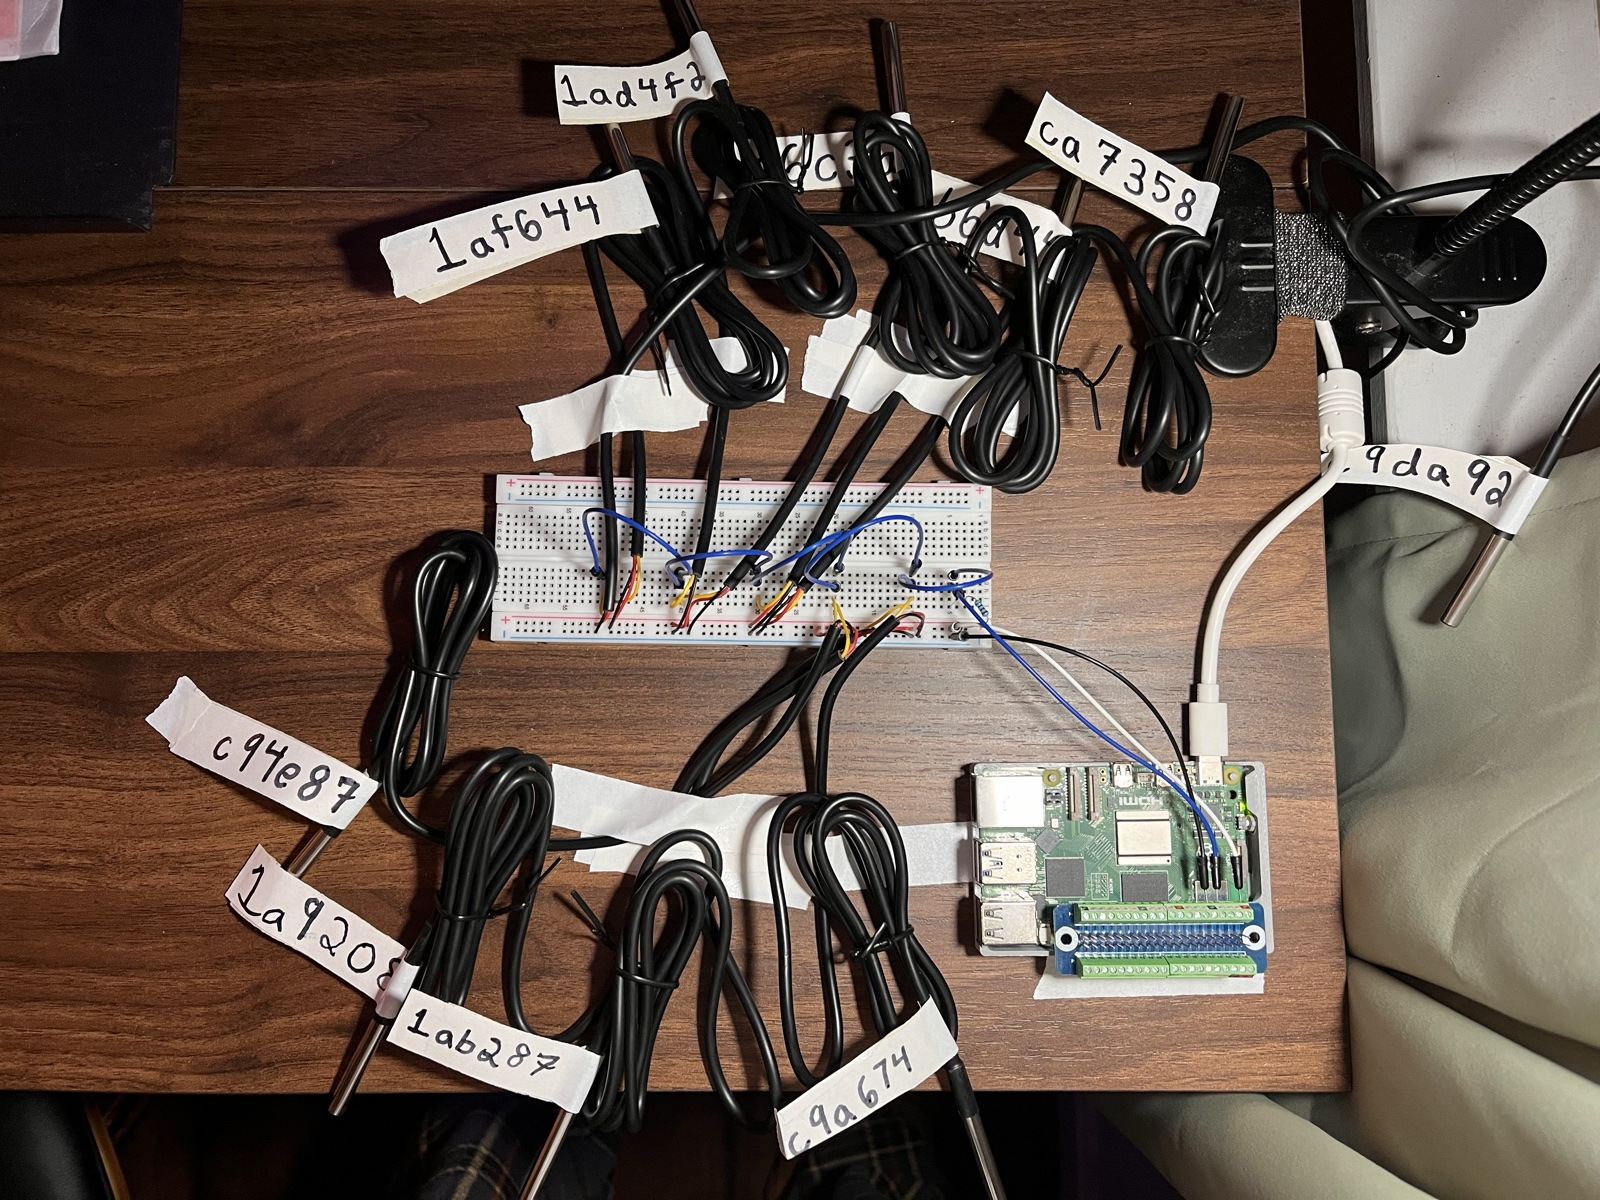
\includegraphics[width=0.32\textwidth]{hardware.jpg}\label{fig:hardware}}
  \hfill
  \subfloat[Breadboard]{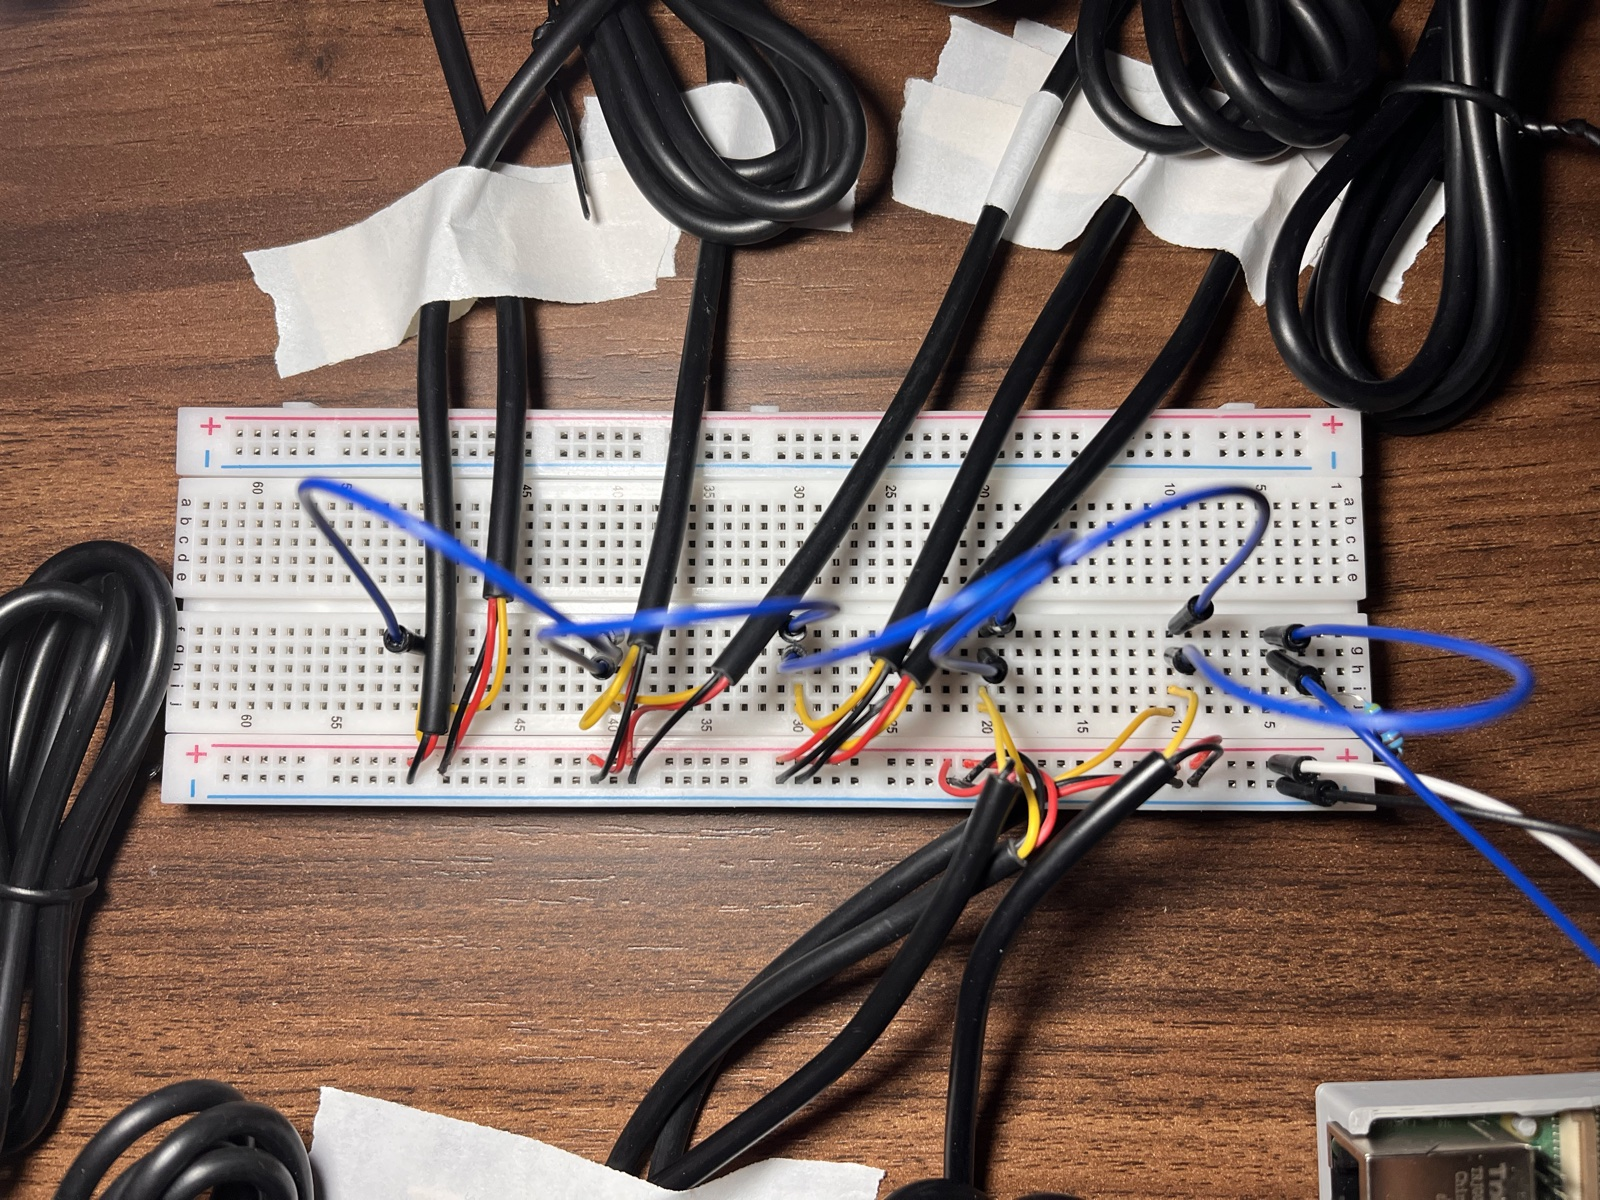
\includegraphics[width=0.32\textwidth]{breadboard.jpg}\label{fig:breadboard}}
  \hfill
  \subfloat[Raspberry Pi 5]{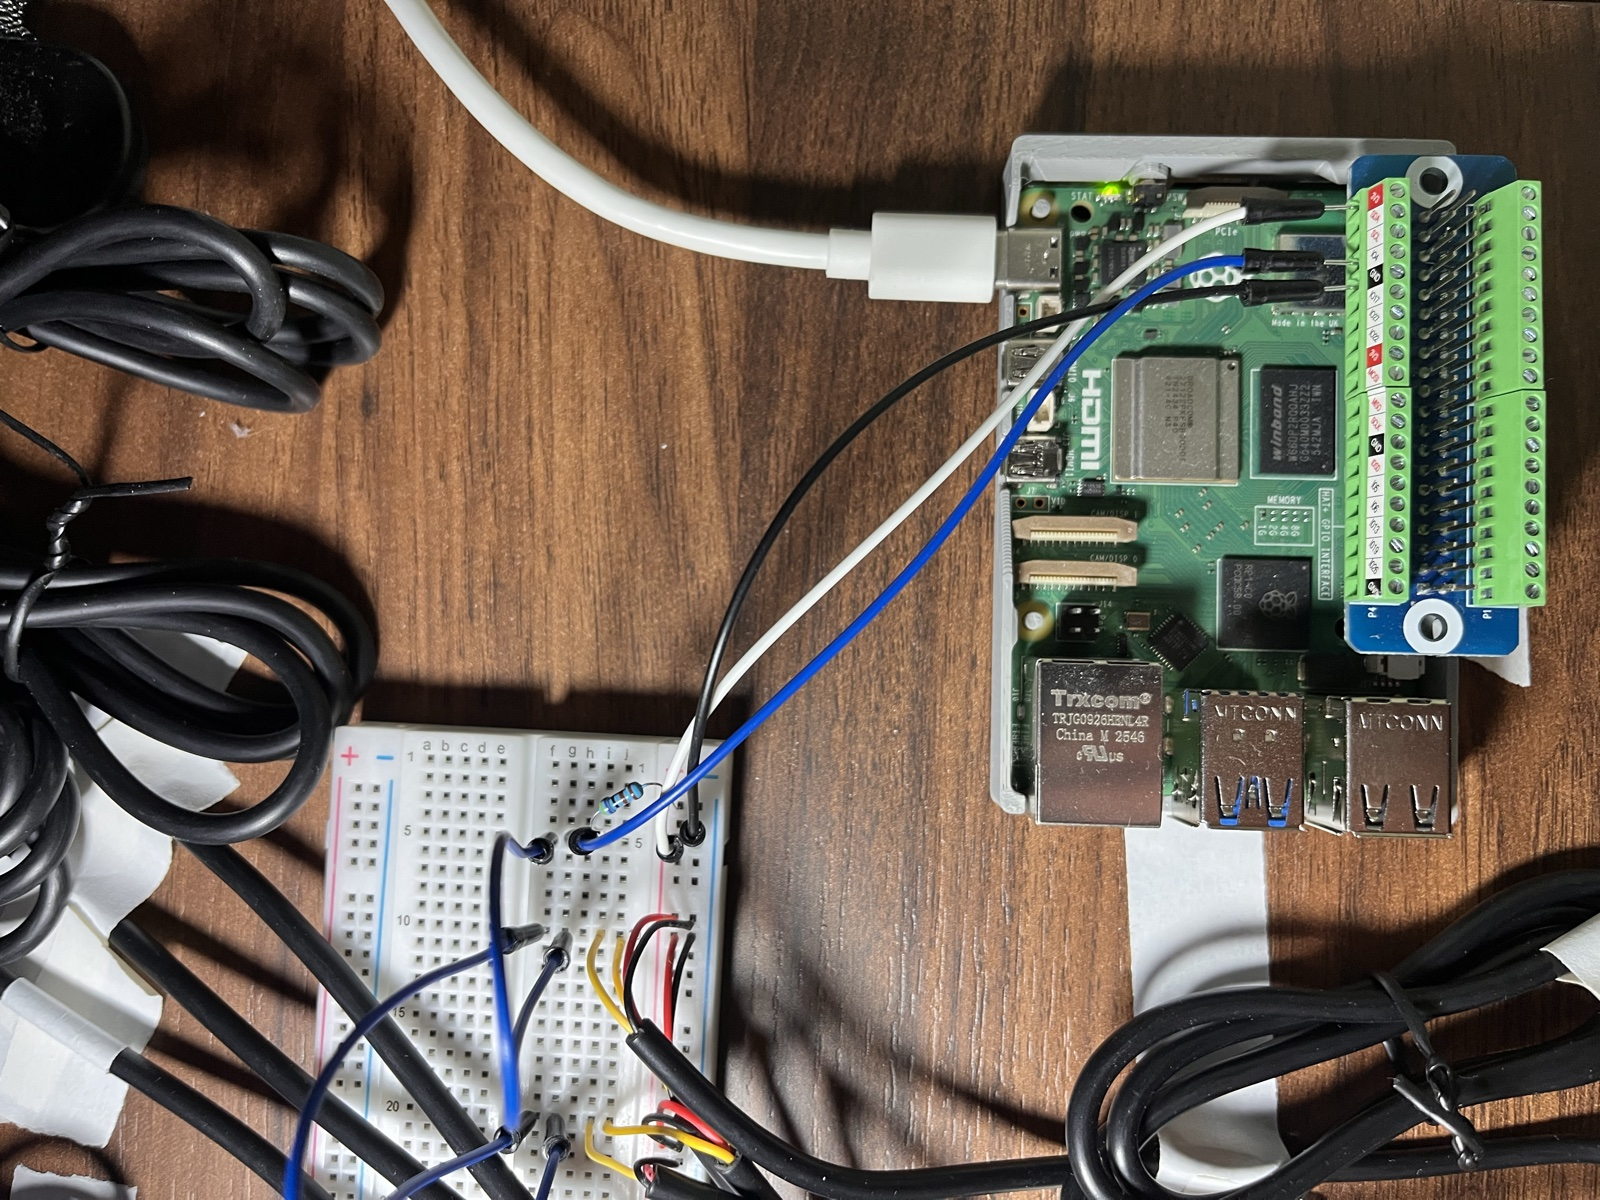
\includegraphics[width=0.32\textwidth]{rpi5.jpg}\label{fig:rpi5}}
  \caption{Test hardware: ten DS18B20 sensors on one w1-gpio bus.}
  \label{fig:setup}
\end{figure*}
% \centerline{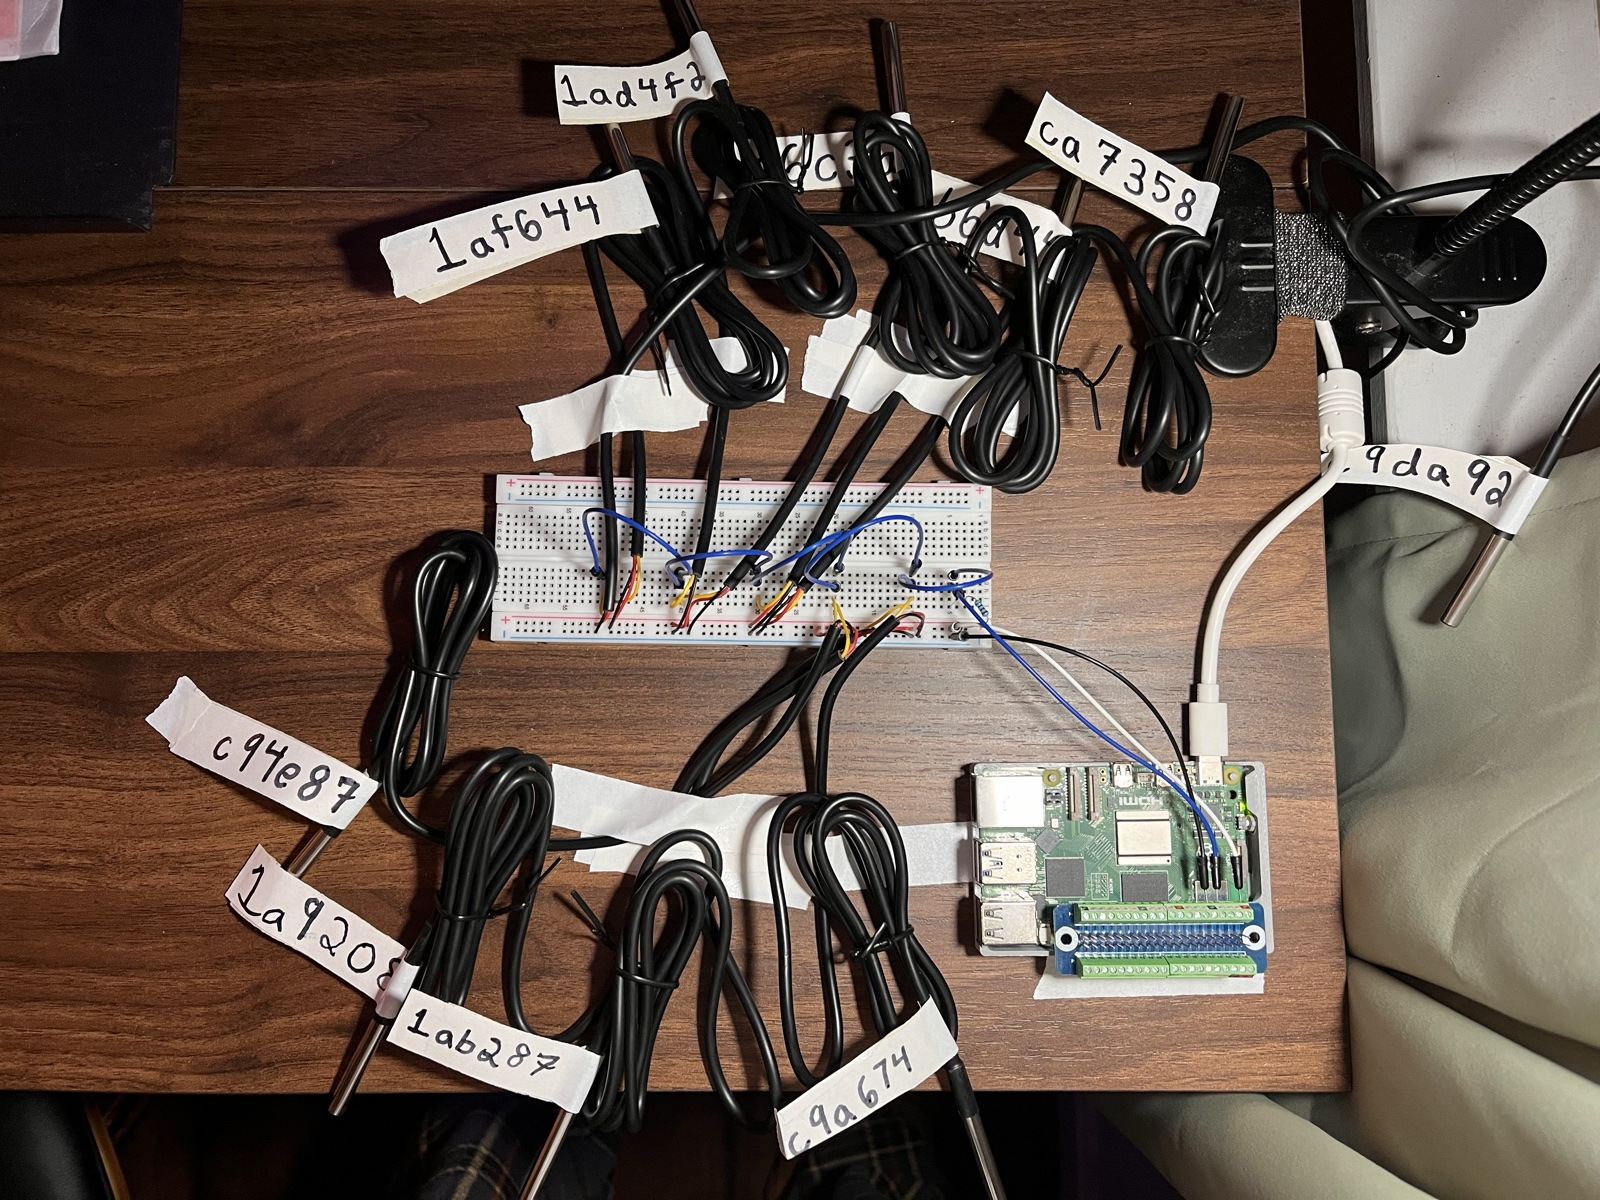
\includegraphics{hardware.jpg}}
% \centerline{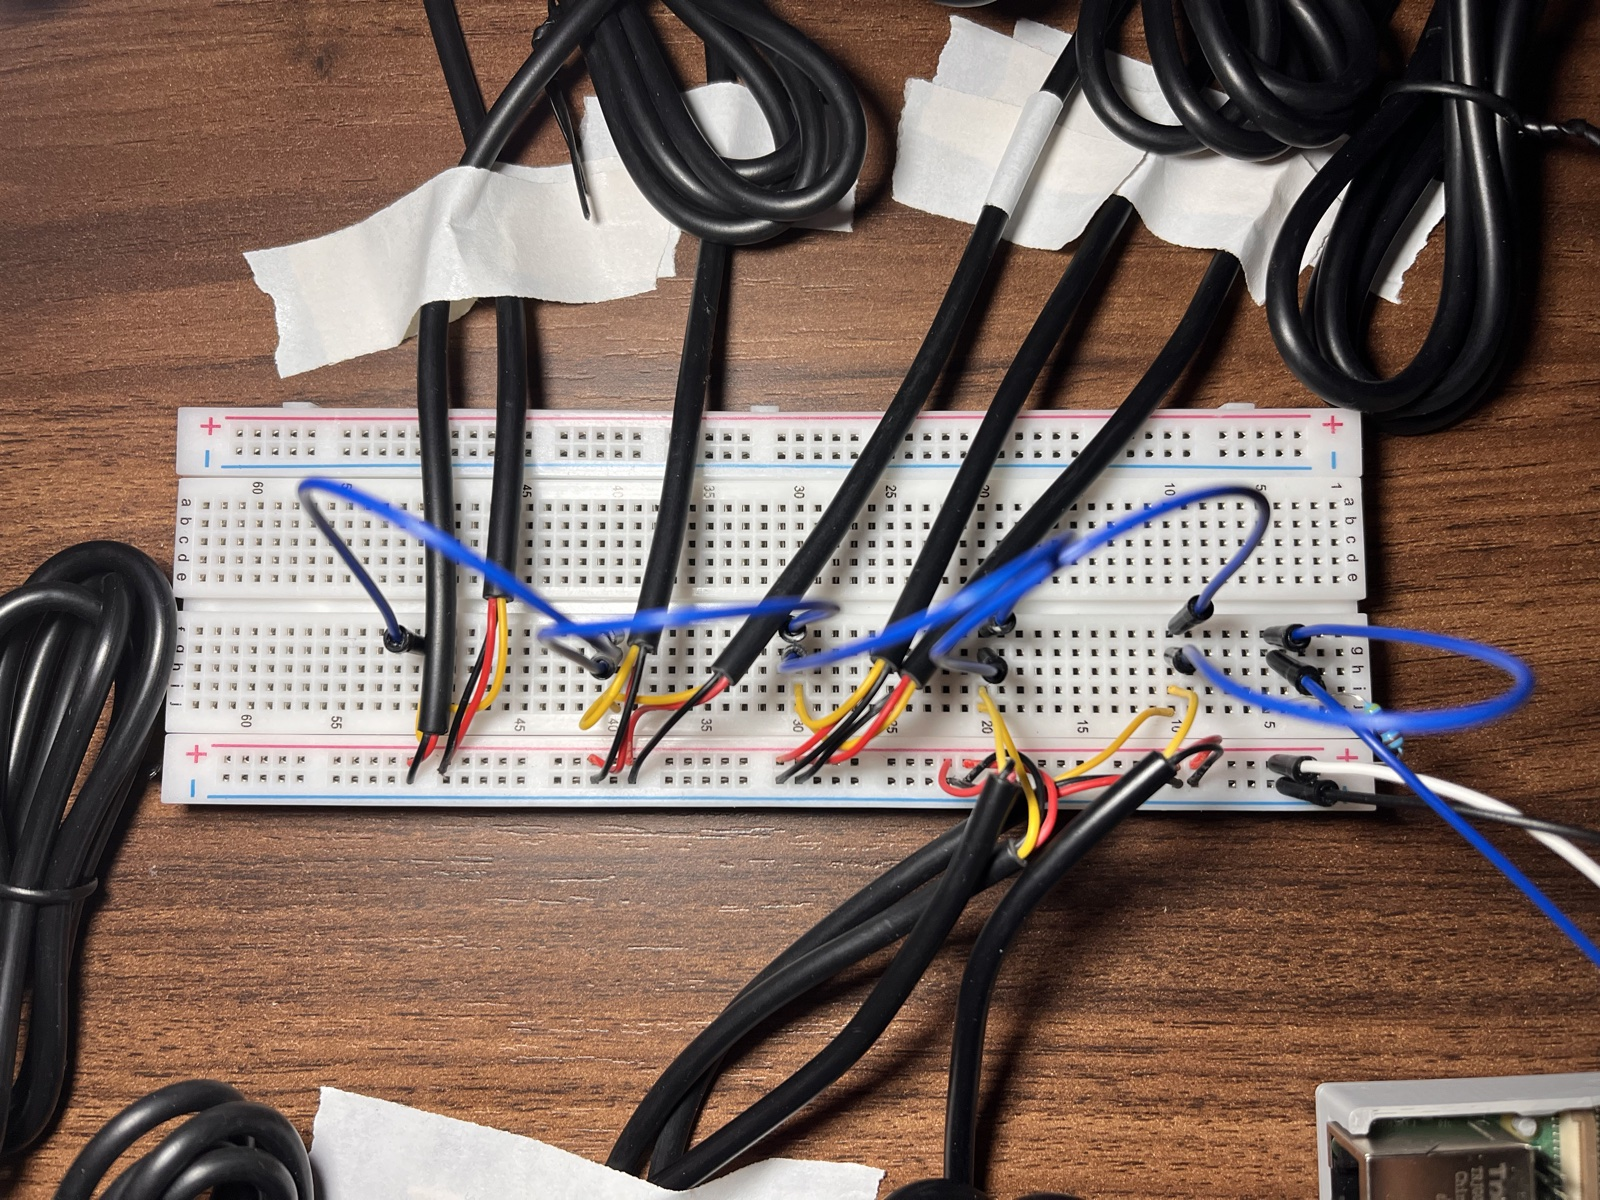
\includegraphics{breadboard.jpg}}
% \centerline{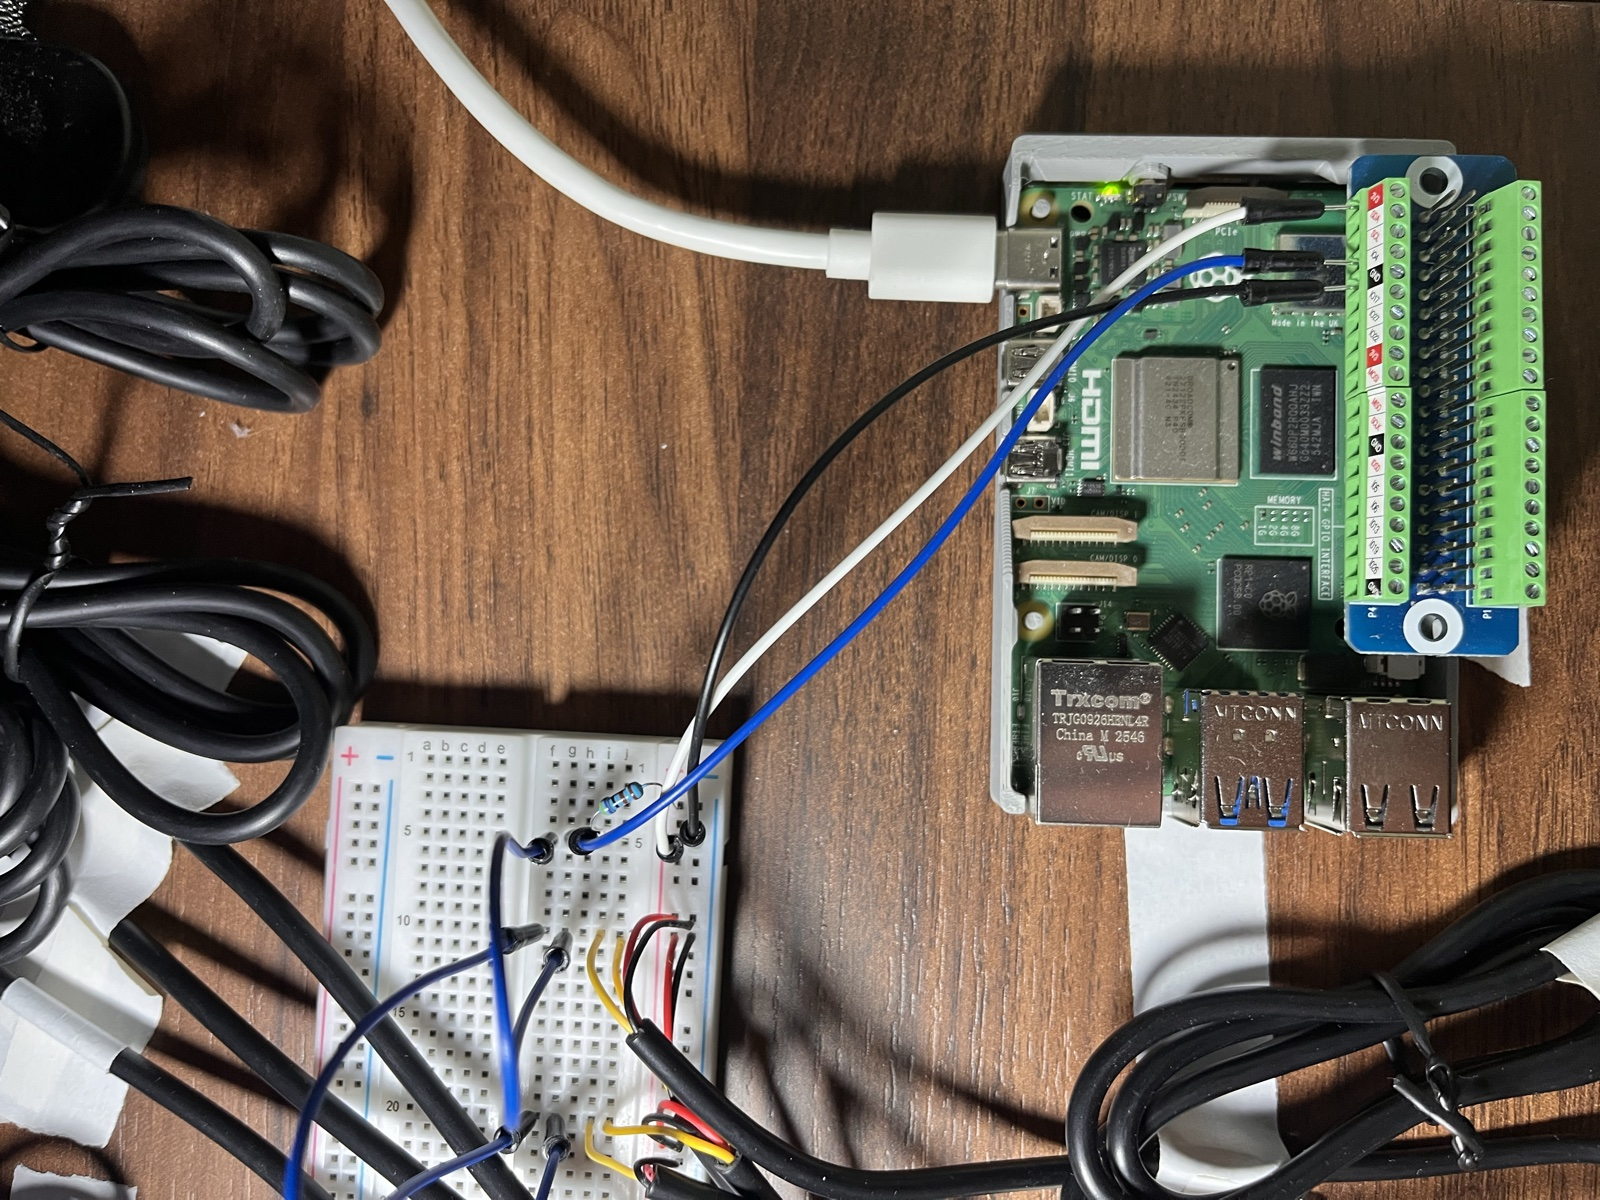
\includegraphics{rpi5.jpg}}

Also include the diagram of the circuit setup here.
\begin{figure*}[t]
  \centering
  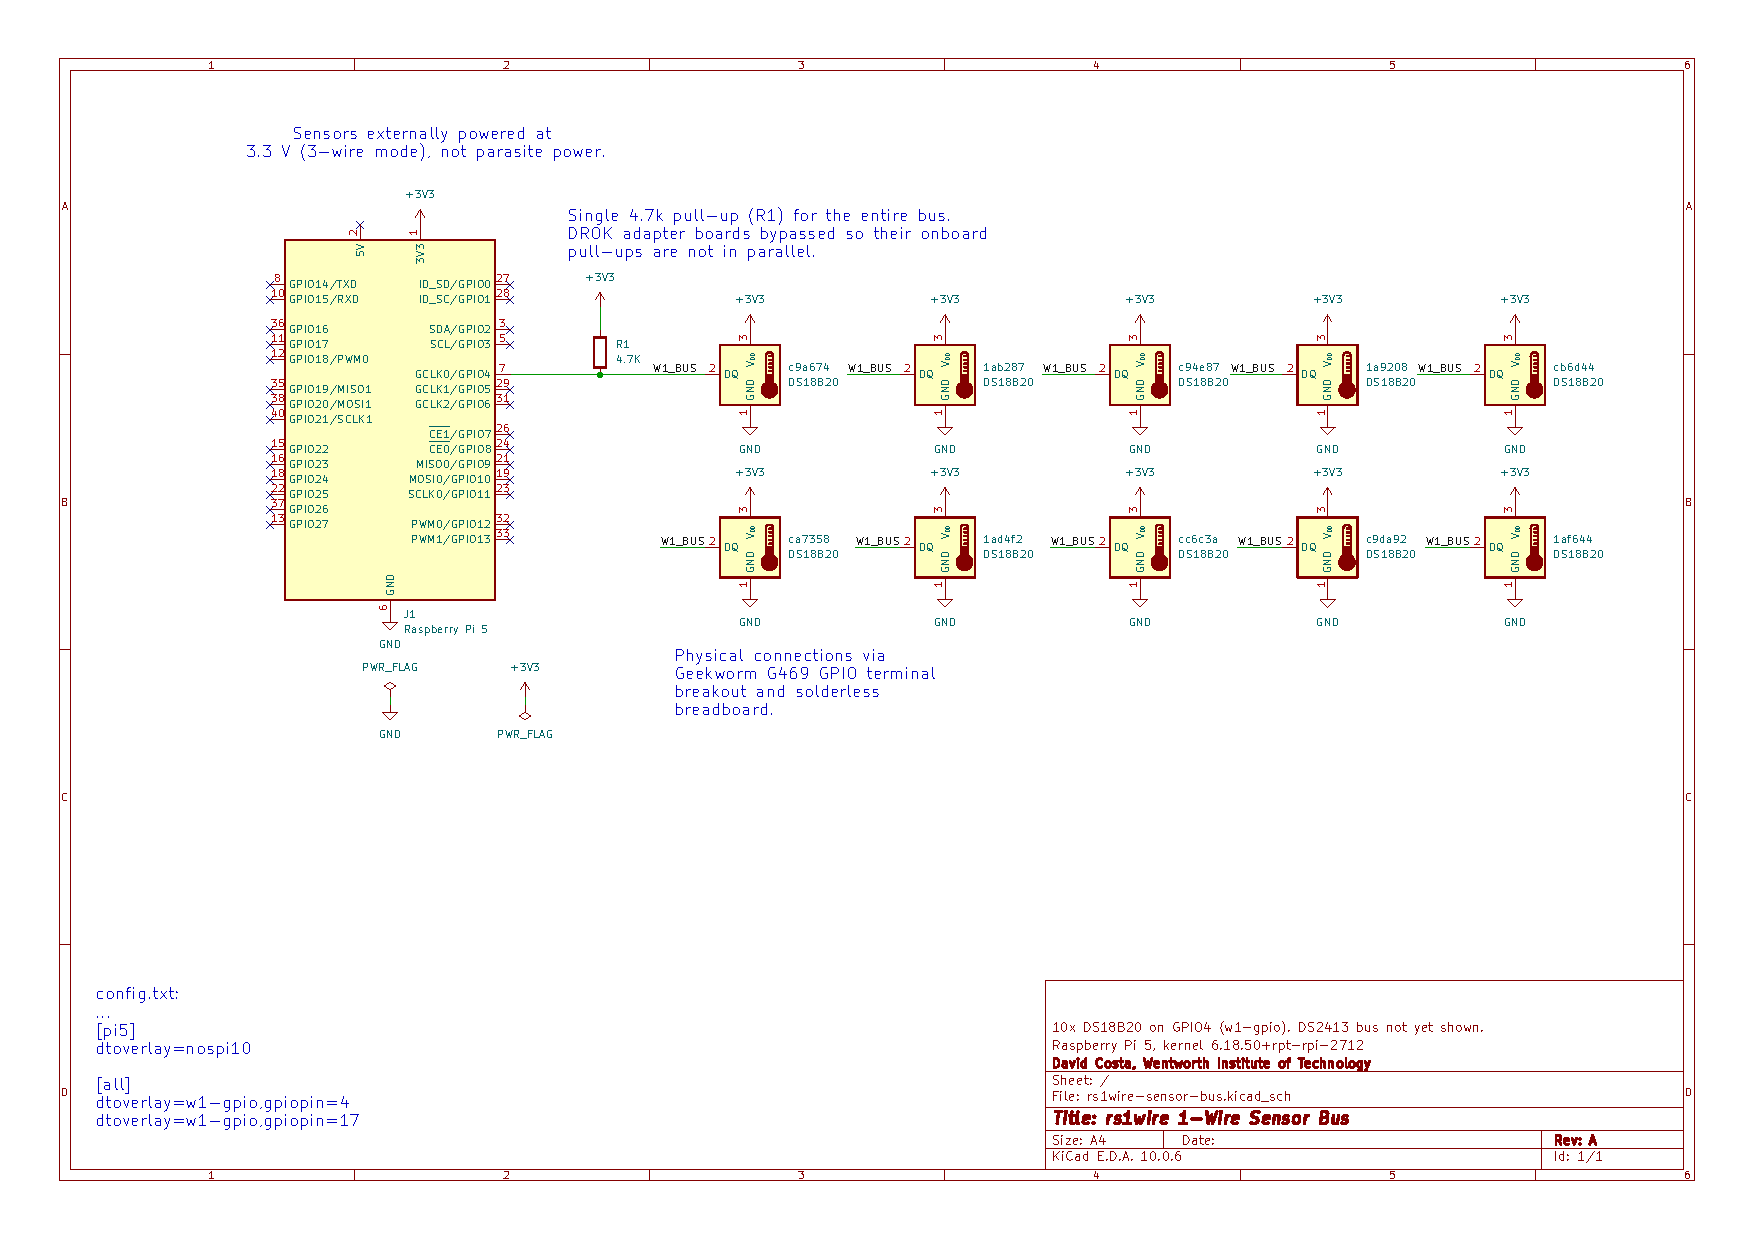
\includegraphics[width=\textwidth]{../hardware/rs1wire-sensor-bus/export/rs1wire-sensor-bus.pdf}
  \caption{Schematic of the 1-Wire sensor bus.}
  \label{fig:circuit}
\end{figure*}


\section*{Results}


\subsection{Figures and Tables}\label{FAT}
\paragraph{Positioning Figures and Tables} Place figures and tables at the top and 
bottom of columns. Avoid placing them in the middle of columns. Large 
figures and tables may span across both columns. Figure captions should be 
below the figures; table heads should appear above the tables. Insert 
figures and tables after they are cited in the text. Use the abbreviation 
``Fig.~\ref{fig}'', even at the beginning of a sentence.

\begin{table}[htbp]
\caption{Table Type Styles}
\begin{center}
\begin{tabular}{|c|c|c|c|}
\hline
\textbf{Table}&\multicolumn{3}{|c|}{\textbf{Table Column Head}} \\
\cline{2-4} 
\textbf{Head} & \textbf{\textit{Table column subhead}}& \textbf{\textit{Subhead}}& \textbf{\textit{Subhead}} \\
\hline
copy& More table copy$^{\mathrm{a}}$& &  \\
\hline
\multicolumn{4}{l}{$^{\mathrm{a}}$Sample of a Table footnote.}
\end{tabular}
\label{tab1}
\end{center}
\end{table}

\begin{figure}[htbp]
%This would be a figure but I deleted the png \centerline{\includegraphics{fig1.png}}
\caption{Example of a figure caption.}
\label{fig}
\end{figure}

Figure Labels: Use 8 point Times New Roman for Figure labels. Use words 
rather than symbols or abbreviations when writing Figure axis labels to 
avoid confusing the reader. As an example, write the quantity 
``Magnetization'', or ``Magnetization, M'', not just ``M''. If including 
units in the label, present them within parentheses. Do not label axes only 
with units. In the example, write ``Magnetization (A/m)'' or ``Magnetization 
\{A[m(1)]\}'', not just ``A/m''. Do not label axes with a ratio of 
quantities and units. For example, write ``Temperature (K)'', not 
``Temperature/K''.


\section*{Discussion}

\section*{Conclusion}

Be sure that the 
symbols in your equation have been defined before or immediately following 
the equation. Use ``\eqref{eq}'', not ``Eq.~\eqref{eq}'' or ``equation \eqref{eq}'', except at 
the beginning of a sentence: ``Equation \eqref{eq} is . . .''

\section*{Acknowledgment}

The author would like to thank all contributors and reviewers for their valuable feedback and support.
Might acknowledge Professor Ashar here? Not sure if he gets his own spot in the author's list or just an acknowledgment as an advisor.
\nocite{*} % list every references.bib entry; remove once the text \cite{}s its sources
\bibliographystyle{IEEEtran}
\bibliography{IEEEabrv,references}
\end{document}
